\paragraph{Generalized operator on separately selected recordings.}
The completed Mac study contains all 26 recordings, both public detector
profiles, 12 bias/cardinality combinations, both query contracts and all
scheduled methods. The independent reconstruction finds maximum curve
discrepancy $2.50\cdot10^{-15}$ and no same-contract winner disagreement.
Table~\ref{tab:weighted-new} reports equal-semantic-weight geometric ratios
against the fused compiled controls. Grid bucketing improves every recording's
aggregate on all three collections. Exhaustive sweep improves all WSD and
Stock aggregates but only one of two MSL recordings. MSL's exhaustive ratios
are .558 and 3.438, so its narrow paired-timing interval around the aggregate
does not indicate robust benefit across new MSL recordings. The separate
recording-reweighting interval [.558,3.438] exposes this sensitivity.
The 12 individual semantic contracts retain the same collection-level
direction: their exhaustive ratios span 8.388--8.959 (WSD), 20.988--23.321
(Stock), and 1.313--1.449 (MSL). Their grid ratios span 1.506--1.549,
1.472--1.714, and 1.519--1.592, respectively. All adjusted paired-order
intervals for these aggregate semantic cells lie above one. Nevertheless,
every MSL exhaustive contract loses on the same one of its two recordings;
the semantic average does not erase that loss. The artifact retains all 36
collection/semantics rows per comparator with both uncertainty summaries.

\begin{table*}[t]\centering\small
\begin{tabular}{llrrr}\toprule
Host & Collection & Grid100 raster/bucket & Distinct raster/sweep & Distinct recording sensitivity\\\midrule
Apple & WSD & 1.526 [1.518,1.530] & 8.801 [8.727,8.837] & [4.896,14.920]\\
Apple & Stock & 1.621 [1.609,1.628] & 22.635 [22.424,22.810] & [17.181,29.800]\\
Apple & MSL & 1.559 [1.542,1.573] & 1.385 [1.362,1.427] & [.558,3.438]\\
Linux & WSD & 2.097 [2.081,2.101] & 7.460 [7.367,7.484] & [4.290,12.454]\\
Linux & Stock & 1.738 [1.734,1.742] & 15.848 [15.628,15.875] & [13.043,19.373]\\
Linux & MSL & 2.072 [2.045,2.090] & 1.670 [1.659,1.682] & [.859,3.244]\\
\bottomrule\end{tabular}
\caption{Original weighted operator study, Apple M1 Pro and fresh Linux replay.
Within each recording,
log ratios are equally weighted across the 12 prespecified bias/cardinality
contracts. Bracketed ratio columns give approximate 95\% paired-order intervals
conditional on this fixed panel, adjusted over three collections. The last
column separately resamples recordings and is workload sensitivity, not a
population confidence interval. WSD and Stock each have 12 recordings; MSL has
two. All ratios compare identical outputs and queries within a row.}
\label{tab:weighted-new}\end{table*}

Sampling has a smaller selection effect on this panel. Only the middle-bias,
cardinality-one contract produces a nonoverlapping grid-versus-exhaustive
winner set, with maximum best-tie regret .001412; no contract produces
best-tie regret .01. A separate post-hoc saved-curve reconstruction finds
singleton grid winners in all 312 case/semantic combinations, so worst-tie
regret is identical on this Mac panel.
Thus the original 15/73 nonoverlap result does not extend as a prevalence
claim to these two unchanged public detectors. The weighted study supports
computational generality while retaining this negative selection result.

\paragraph{Fresh Linux execution.}
The original fresh replay verifies the raw archive,
425 TimeEval source files and all typed inputs, regenerates 52 detector
profiles, and reconstructs both operator and consumer outputs. Compared with
Mac, all 26 label-array hashes agree but 25/52 score hashes differ, all from
COPOD; FFT's 26 score hashes agree. These are independently generated host
workloads, not an isolated CPU intervention. Native query totals are 2,776
at the nominal default on both hosts and 71,749/71,750 at all observed queries
on Mac/Linux. No timing or uncertainty is pooled across hosts.
The Linux weighted study reconstructs all 11,232 records and 156 curves,
with maximum error $2.50\cdot10^{-15}$ and zero same-contract winner
disagreements. Table~\ref{tab:weighted-new} gives its aggregate results.
Linux MSL id7 loses against exhaustive raster (.859) and against grid sweep
(.963); ten of the MSL collection-level grid sweep/bucket semantic intervals
include one. Thus the Mac semantic result is not asserted uniformly across
Linux contracts. All 312 Linux grid winner sets are also singletons; the
largest best/worst-tie regret remains .001412, with none reaching .01.

\paragraph{Native public consumer.}
The Mac execution completes 120 of 144 scheduled records, with four public
600-second censors and 20 prespecified skips. The independent auditor verifies
all completed CSVs and reconstructs maximum scalar discrepancy
$3.33\cdot10^{-16}$. Completed public outputs cover 28/52 profiles in each
contract (MSL and WSD); Stock has compiled-to-compiled agreement only. Matching
family outputs also verify those same profiles in the combined batch, but do
not supply its censored public execution time.

Table~\ref{tab:native-mac} shows absolute whole-workflow medians and matched
compiled comparisons. At all observed queries, the combined raster/bucket
ratio is 2.728 [2.649,2.801], including native loading, three metrics and result
writing. At the nominal default it is 1.017 [.998,1.039], with no supported
advantage over raster. Public-code engineering gains are much larger: completed
WSD public/bucket ratios are 9.598 [9.438,9.774] at the default and
407.099 [398.649,416.713] at all observed queries. These are not all attributable
to the incremental recurrence. The separately frozen interval control below
tests the remaining conventional-algorithm explanation.

\begin{table*}[t]\centering\small
\begin{tabular}{llrrrr}\toprule
Query contract & Batch (profiles) & Public seconds & Raster seconds & Bucket seconds & Raster/bucket [95\% interval]\\\midrule
Nominal 50 & All (52) & censored $>600$ & 1.0848 & 1.0783 & 1.017 [.998,1.039]\\
Nominal 50 & MSL (4) & .08008 & .03177 & .03291 & .860 [.639,1.014]\\
Nominal 50 & Stock (24) & censored $>600$ & .48931 & .48169 & 1.043 [1.013,1.083]\\
Nominal 50 & WSD (24) & 5.22731 & .55475 & .54321 & 1.019 [1.003,1.037]\\
All observed & All (52) & censored $>600$ & 2.94605 & 1.08068 & 2.728 [2.649,2.801]\\
All observed & MSL (4) & .48152 & .03352 & .03038 & 1.088 [1.045,1.136]\\
All observed & Stock (24) & censored $>600$ & 1.86034 & .50496 & 3.557 [3.354,3.715]\\
All observed & WSD (24) & 234.80063 & 1.07523 & .58478 & 1.866 [1.832,1.901]\\
\bottomrule\end{tabular}
\caption{Native TimeEval read-to-result-write execution on Apple M1 Pro.
Absolute times are medians of six completed workflows. Ratios are geometric
means of six matched-order ratios, not ratios of the displayed medians;
intervals are approximate conditional paired-order intervals. Each censored
public key has one timeout and five unrun repetitions, not a completed median
or interval. The native nominal/all-observed contracts emit 2,776/71,749 queries
across 52 profiles; no cross-contract speed ratio is asserted.}
\label{tab:native-mac}\end{table*}

The original fresh Linux replay also completes 120 workflows, with four
600-second public censors and 20 prescribed skips. It verifies public outputs
for the same 28/52 profiles per contract, with maximum discrepancy
$3.33\cdot10^{-16}$. Table~\ref{tab:native-linux} retains all batch results.
The combined exhaustive raster/bucket ratio is 1.932 [1.907,1.946], smaller
than the separately executed conventional-control replay below. Its default
ratio is 1.014 [1.007,1.027], a small benefit that is not consistently supported
by the other runs' intervals. MSL's exhaustive aggregate does not support a
gain; one bucket trial takes .09497 seconds, versus .04342--.04491 for its
other five trials. That observation is retained, not removed as an outlier.

\begin{table*}[t]\centering\small
\begin{tabular}{llrrrr}\toprule
Query contract & Batch (profiles) & Public seconds & Raster seconds & Bucket seconds & Raster/bucket [95\% interval]\\\midrule
Nominal 50 & All (52) & censored $>600$ & 1.58408 & 1.56792 & 1.014 [1.007,1.027]\\
Nominal 50 & MSL (4) & .25969 & .04442 & .04485 & .992 [.986,.9997]\\
Nominal 50 & Stock (24) & censored $>600$ & .71023 & .70782 & 1.020 [1.003,1.046]\\
Nominal 50 & WSD (24) & 14.44195 & .83543 & .82163 & 1.027 [1.015,1.050]\\
All observed & All (52) & censored $>600$ & 3.04217 & 1.56594 & 1.932 [1.907,1.946]\\
All observed & MSL (4) & 1.94251 & .04737 & .04445 & .941 [.730,1.076]\\
All observed & Stock (24) & censored $>600$ & 1.68294 & .70907 & 2.342 [2.280,2.377]\\
All observed & WSD (24) & 406.24099 & 1.33226 & .84578 & 1.577 [1.559,1.593]\\
\bottomrule\end{tabular}
\caption{Original public-reference TimeEval replay on Linux. Timing, ratio,
censor and uncertainty definitions match Table~\ref{tab:native-mac}; native
query totals are 2,776/71,750. Stock and combined public calls have no completed
median. All completed trials, including the slower MSL bucket trial, enter
the reported estimates.}\label{tab:native-linux}\end{table*}

\paragraph{Conventional interval control.}
The separately frozen ablation compares incremental curves with closed-form
interval recomputation and remeasures raster on the same panel. Its fresh Linux
run regenerates all 52 public profiles before timing. Both hosts complete all
scheduled weighted cases and 144 native workflows. Maximum weighted curve
discrepancy is $2.39\cdot10^{-15}$ on each host; native scalar discrepancy is at most
$3.33\cdot10^{-16}$ on each host. Table~\ref{tab:interval-control} gives the
interval comparisons. Every collection/query aggregate favors incremental
evaluation, but interval is not uniformly the fastest conventional control:
raster/interval aggregate ratios are below one in five of six Mac comparisons
and all six Linux comparisons. Both controls remain visible.

\begin{table*}[t]\centering\small
\begin{tabular}{llrrr}\toprule
Host & Collection & Grid100 interval/bucket & Distinct interval/sweep & Distinct recording sensitivity\\\midrule
Apple & WSD & 1.665 [1.658,1.671] & 7.323 [7.277,7.342] & [4.290,11.919]\\
Apple & Stock & 2.051 [2.040,2.059] & 26.339 [26.244,26.387] & [19.472,35.575]\\
Apple & MSL & 1.753 [1.725,1.759] & 1.706 [1.679,1.728] & [.775,3.759]\\
Linux & WSD & 2.308 [2.293,2.315] & 12.945 [12.396,12.991] & [7.566,21.139]\\
Linux & Stock & 2.289 [2.282,2.296] & 36.149 [35.977,36.224] & [27.994,46.863]\\
Linux & MSL & 2.331 [2.306,2.348] & 2.381 [2.347,2.418] & [1.024,5.536]\\
\bottomrule\end{tabular}
\caption{Prospectively frozen conventional-interval ablation. Both controls
and the incremental method share compiler and output semantics. Interval
recomputation uses closed-form overlap at each query and no cross-query metric
state. The paired-order and recording-sensitivity intervals have the same
interpretation as Table~\ref{tab:weighted-new}; they are not pooled across hosts.
Remeasured raster results and all 12 individual semantic contracts are retained
in the artifact.}\label{tab:interval-control}
\end{table*}

On Mac, all 72 collection/semantic/query intervals against interval control
lie above one, but MSL id7 loses every exhaustive semantic setting
(aggregate .775), while id3 improves 3.759 times. On Linux, id7 improves only
1.024 times over interval; the faster raster still limits the benefit.
The conditional aggregate intervals therefore do not establish uniformly
positive performance on new recordings.

A separate exploratory post-hoc contrast directly reconstructs raster over
incremental from the same supplemental trials, with paired-order tails adjusted
over all six collection/query contrasts per host. Exhaustive ratios are
8.608 [8.549,8.639], 21.991 [21.908,22.050] and 1.421 [1.403,1.461] on Mac,
and 11.621 [11.111,11.668], 26.717 [26.579,26.786] and
1.726 [1.695,1.776] on Linux, in WSD/Stock/MSL order.
These exploratory intervals do not correct post-hoc comparator selection.
The fixed-raster contrast retains MSL id7's loss on both hosts;
Figure~\ref{fig:query-regime} also displays the faster of the two conventional
controls per recording without assigning an interval to this lower envelope.

\begin{figure*}[t]\centering
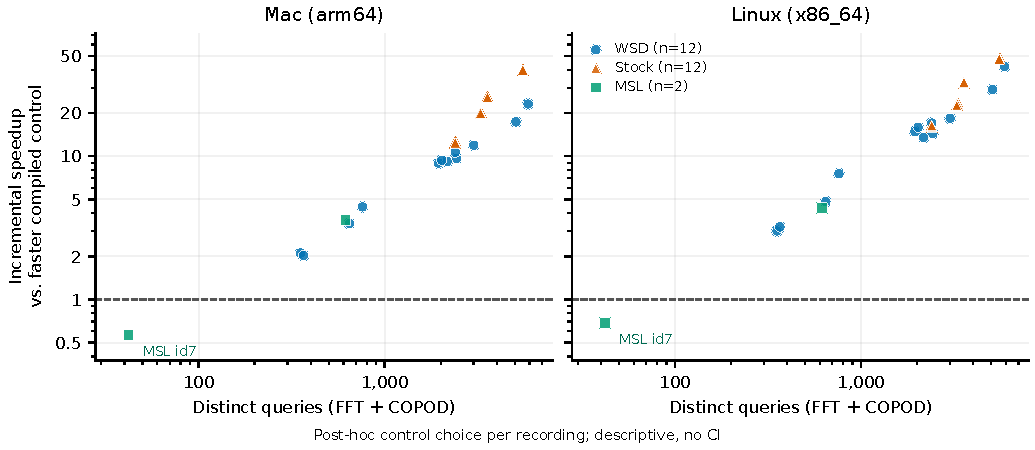
\includegraphics[width=.94\textwidth]{../artifacts/pvldb-research-20261024/strengthening/figures/interval-control-two-host-v1/interval-control-query-regime.pdf}
\caption{Post-hoc descriptive query-regime view of the supplemental study.
Each point is one recording, equally weighting its 12 semantic log ratios.
The denominator is incremental evaluation; the numerator selects the faster
geometric aggregate of raster and interval for that recording. This is a
descriptive lower envelope of measured controls, not a deployable selector or
a prespecified confidence interval. MSL id7 loses on both hosts. Distinct
query counts sum the two public detector profiles.}
\label{fig:query-regime}
\end{figure*}

The native conventional-control ablation retains complete three-metric
read-to-write semantics. At all observed queries, combined interval/bucket
ratios are 3.034 [2.990,3.075] on Mac and 3.190 [3.166,3.224] on Linux.
The faster combined raster control gives 2.732 [2.656,2.812] and
2.756 [2.742,2.773], respectively. At default sampling, raster/bucket is only
1.026 [.998,1.049] and 1.016 [.997,1.033]. Thus the exhaustive-workflow gain
survives the additional control on both hosts, while neither host supports a
default combined-workflow gain over raster. These compiled-only trials add no
public-reference coverage to the earlier study.
\begin{table*}[t]\centering\small
\begin{tabular}{llrrrrr}\toprule
Host & Queries & Raster s & Interval s & Bucket s & Raster/bucket & Interval/bucket\\\midrule
Apple & Nominal 50 & 1.0686 & 1.0991 & 1.0429 & 1.026 [0.998,1.049] & 1.043 [1.016,1.067]\\
Apple & All observed & 2.9474 & 3.2754 & 1.0726 & 2.732 [2.656,2.812] & 3.034 [2.990,3.075]\\
Linux & Nominal 50 & 1.4617 & 1.4880 & 1.4381 & 1.016 [0.997,1.033] & 1.034 [1.015,1.047]\\
Linux & All observed & 4.1126 & 4.7551 & 1.4990 & 2.756 [2.742,2.773] & 3.190 [3.166,3.224]\\
\bottomrule\end{tabular}
\caption{Combined native TimeEval workflows in the separately frozen conventional-control study. Each row evaluates all 52 profiles and all three metrics from CSV read to result write/close. Absolute times are medians of six runs; paired ratios and conditional intervals are independently reconstructed from matched orders. These compiled-only runs supply no additional public-reference coverage.}\label{tab:native-control}
\end{table*}


Across all four original/supplemental Apple/Linux executions, the combined
exhaustive raster/bucket ratio spans 1.932--2.756; results are not pooled.
The two Linux runs have identical hashes for all 52 score profiles and the
shared sources, but their recorded OpenBLAS dispatch architectures differ
(Cooperlake versus SkylakeX). The supplemental combined raster median is
35.2\% higher and bucket median 4.3\% lower than in the original run. These
descriptive differences do not identify a causal CPU or load effect. The
narrow paired-order intervals are conditional within each run and do not
cover this between-run variability.

The same tables give a descriptive cost--fidelity observation, rather than a
same-output speed ratio. Moving from the native nominal default to all observed
queries increases query count from 2,776 to 71,749/71,750 on Mac/Linux, while
the incremental combined workflow's median changes from 1.043 to 1.073 seconds
and from 1.438 to 1.499 seconds. This workload can therefore obtain the complete
native query close to its sampled workflow cost. These are warm-workflow
medians under different query contracts, not paired timing intervals or evidence
of a practically important detector-selection improvement.

The per-collection native results retain practical counterexamples. At default
sampling, Linux MSL favors raster (.981 [.973,.988] raster/bucket), while
Stock's .997 [.967,1.018] interval crosses one. At all observed queries,
interval/bucket on Linux is 1.256 [1.090,1.643] for MSL,
4.649 [4.632,4.666] for Stock and 1.897 [1.849,1.932] for WSD.
The conventional-control ordering for exhaustive WSD changes across hosts:
raster/interval is 1.073 on Mac but .961 on Linux. Reporting only the
slower conventional implementation would overstate the joint-state increment.
